\chapter{Evaluation\label{cha:chapter5}}

This chapter describes the evaluation method and results for the developed software solutions. 
The evaluation is divided into three main sections: 
\begin{itemize}
    \item Functional Evaluation
    \item Performance Evaluation
    \item Edge cases Analysis
\end{itemize}

All the test has been executed on the same machine, with the same configuration. \paragraph{Test Environment} Intel Core i7, 16 GB RAM, MacOS 15.4.1 

    

% Start 

\section{Functional Evaluation}

\subsection{Instance Generation}

\paragraph{Goal}
The first core functionality to evaluate is the \textbf{automatic generation of RDF instances}. This feature assist users by generating RDF instances based on a given RDF schema .

\paragraph{Test Description}
To validate this capability, two test scenarios were conducted:
\begin{itemize}
    \item \textbf{Test 1.1}: Generate instances from an RDF schema without additional properties.
    \item \textbf{Test 1.2}: Generate instances from an RDF schema and search for additional properties.
\end{itemize}

\subsubsection{Expected Result}

In the first case, the system was expected to:
\begin{itemize}
    \item Correctly generate RDF instances for each class.
    \item Ensure that instances respect domain and range restrictions.
    \item Keep the schema original schema structure intact, without any modifications in the classes or properties definitions.
\end{itemize}

In the second case, the system was expected to:
\begin{itemize}
    \item Correctly generate RDF instances for each class.
    \item Correctly generate additional properties for instance of non-implicitly referolive classes. 
    \item Ensure that instances respect domain and range restrictions.
    \item Keep the schema original schema structure intact, without any modifications in the classes or properties definitions.
\end{itemize}


\paragraph{Test Environment}
\begin{itemize}
    \item Test device: Intel Core i7, 16 GB RAM, MacOS 15.4.1 
\end{itemize}

\subsubsection{Actual Results}

The following two code sample, are the results of the two tests cases. For both the cases, the same RDF schema was provided. The code lines highlighted in olive green represent the synthetic instances generated by system. Three new instances were requested to be generated.
\\
Each of them has been marked as passed.
\\
\begin{lstlisting}[caption={Result Test Case 1.1}, label={lst:three-rdf-instances}]
    @prefix ex: <http://example.org/> .
    @prefix foaf: <http://xmlns.com/foaf/0.1/> .
    @prefix rdf: <http://www.w3.org/1999/02/22-rdf-syntax-ns#> .
    @prefix rdfs: <http://www.w3.org/2000/01/rdf-schema#> .
    @prefix schema1: <http://schema.org/> .
    @prefix xsd: <http://www.w3.org/2001/XMLSchema#> .
    
    ex:Employee a rdfs:Class ;
        rdfs:label "Employee" ;
        rdfs:comment "A class representing an employee." ;
        rdfs:subClassOf foaf:Person .
    
    (*@\textcolor{olive}{ex:Employee\_Instance1 a ex:Employee ;}@*)
        (*@\textcolor{olive}{ex:age 0 ;}@*)
        (*@\textcolor{olive}{ex:hasCar ex:Car\_Instance1 ;}@*)
        (*@\textcolor{olive}{ex:hasProfilePic ex:Image\_Instance1 ;}@*)
        (*@\textcolor{olive}{ex:isAtHome false ;}@*)
        (*@\textcolor{olive}{ex:ishuman "unknown"\textasciicircum{}\textasciicircum{}xsd:string .}@*)
    
    (*@\textcolor{olive}{ex:Employee\_Instance2 a ex:Employee ;}@*)
        (*@\textcolor{olive}{ex:age 0 ;}@*)
        (*@\textcolor{olive}{ex:hasCar ex:Car\_Instance2 ;}@*)
        (*@\textcolor{olive}{ex:hasProfilePic ex:Image\_Instance2 ;}@*)
        (*@\textcolor{olive}{ex:isAtHome false ;}@*)
        (*@\textcolor{olive}{ex:ishuman "unknown"\textasciicircum{}\textasciicircum{}xsd:string .}@*)
    
    (*@\textcolor{olive}{ex:Employee\_Instance3 a ex:Employee ;}@*)
        (*@\textcolor{olive}{ex:age 0 ;}@*)
        (*@\textcolor{olive}{ex:hasCar ex:Car\_Instance3 ;}@*)
        (*@\textcolor{olive}{ex:hasProfilePic ex:Image\_Instance3 ;}@*)
        (*@\textcolor{olive}{ex:isAtHome false ;}@*)
        (*@\textcolor{olive}{ex:ishuman "unknown"\textasciicircum{}\textasciicircum{}xsd:string .}@*)
    
    (*@\textcolor{olive}{ex:Person\_Instance1 a foaf:Person .}@*)
    
    (*@\textcolor{olive}{ex:Person\_Instance2 a foaf:Person .}@*)
    
    (*@\textcolor{olive}{ex:Person\_Instance3 a foaf:Person .}@*)
    
    ex:age a rdf:Property ;
        rdfs:domain ex:Employee ;
        rdfs:range xsd:integer .
    
    ex:hasCar a rdf:Property ;
        rdfs:label "hasCar" ;
        rdfs:comment "A property linking an employee to their car." ;
        rdfs:domain ex:Employee ;
        rdfs:range schema1:Car .
    
    ex:hasProfilePic a rdf:Property ;
        rdfs:domain ex:Employee ;
        rdfs:range foaf:Image .
    
    ex:isAtHome a rdf:Property ;
        rdfs:domain ex:Employee ;
        rdfs:range xsd:boolean .
    
    ex:ishuman a rdf:Property ;
        rdfs:domain ex:Employee ;
        rdfs:range xsd:string .
    
    (*@\textcolor{olive}{ex:Car\_Instance1 a schema1:Car .}@*)
    
    (*@\textcolor{olive}{ex:Car\_Instance2 a schema1:Car .}@*)
    
    (*@\textcolor{olive}{ex:Car\_Instance3 a schema1:Car .}@*)
    
    (*@\textcolor{olive}{ex:Image\_Instance1 a foaf:Image .}@*)
    
    (*@\textcolor{olive}{ex:Image\_Instance2 a foaf:Image .}@*)
    
    (*@\textcolor{olive}{ex:Image\_Instance3 a foaf:Image .}@*)
    \end{lstlisting}

    \begin{lstlisting}[caption={Result Test Case 1.2}, label={lst:three-rdf-instances-extended}]
@prefix ex: <http://example.org/> .
@prefix foaf: <http://xmlns.com/foaf/0.1/> .
@prefix rdf: <http://www.w3.org/1999/02/22-rdf-syntax-ns#> .
@prefix rdfs: <http://www.w3.org/2000/01/rdf-schema#> .
@prefix schema1: <http://schema.org/> .
@prefix xsd: <http://www.w3.org/2001/XMLSchema#> .

ex:Employee a rdfs:Class ;
    rdfs:label "Employee" ;
    rdfs:comment "A class representing an employee." ;
    rdfs:subClassOf foaf:Person .

(*@\textcolor{olive}{ex:Employee\_Instance1 a ex:Employee ;}@*)
    (*@\textcolor{olive}{ex:age 0 ;}@*)
    (*@\textcolor{olive}{ex:hasCar ex:Car\_Instance1 ;}@*)
    (*@\textcolor{olive}{ex:hasProfilePic ex:Image\_Instance1 ;}@*)
    (*@\textcolor{olive}{ex:isAtHome false ;}@*)
    (*@\textcolor{olive}{ex:ishuman "unknown"\textasciicircum{}\textasciicircum{}xsd:string .}@*)

(*@\textcolor{olive}{ex:Employee\_Instance2 a ex:Employee ;}@*)
    (*@\textcolor{olive}{ex:age 0 ;}@*)
    (*@\textcolor{olive}{ex:hasCar ex:Car\_Instance2 ;}@*)
    (*@\textcolor{olive}{ex:hasProfilePic ex:Image\_Instance2 ;}@*)
    (*@\textcolor{olive}{ex:isAtHome false ;}@*)
    (*@\textcolor{olive}{ex:ishuman "unknown"\textasciicircum{}\textasciicircum{}xsd:string .}@*)

(*@\textcolor{olive}{ex:Employee\_Instance3 a ex:Employee ;}@*)
    (*@\textcolor{olive}{ex:age 0 ;}@*)
    (*@\textcolor{olive}{ex:hasCar ex:Car\_Instance3 ;}@*)
    (*@\textcolor{olive}{ex:hasProfilePic ex:Image\_Instance3 ;}@*)
    (*@\textcolor{olive}{ex:isAtHome false ;}@*)
    (*@\textcolor{olive}{ex:ishuman "unknown"\textasciicircum{}\textasciicircum{}xsd:string .}@*)

(*@\textcolor{olive}{ex:Person\_Instance1 a foaf:Person ;}@*)
    (*@\textcolor{olive}{foaf:name "FedX" .}@*)

(*@\textcolor{olive}{ex:Person\_Instance2 a foaf:Person ;}@*)
    (*@\textcolor{olive}{foaf:name "FedX" .}@*)

(*@\textcolor{olive}{ex:Person\_Instance3 a foaf:Person ;}@*)
    (*@\textcolor{olive}{foaf:name "FedX" .}@*)

ex:age a rdf:Property ;
    rdfs:domain ex:Employee ;
    rdfs:range xsd:integer .

ex:hasCar a rdf:Property ;
    rdfs:label "hasCar" ;
    rdfs:comment "A property linking an employee to their car." ;
    rdfs:domain ex:Employee ;
    rdfs:range schema1:Car .

ex:hasProfilePic a rdf:Property ;
    rdfs:domain ex:Employee ;
    rdfs:range foaf:Image .

ex:isAtHome a rdf:Property ;
    rdfs:domain ex:Employee ;
    rdfs:range xsd:boolean .

ex:ishuman a rdf:Property ;
    rdfs:domain ex:Employee ;
    rdfs:range xsd:string .

(*@\textcolor{olive}{ex:Car\_Instance1 a schema1:Car ;}@*)
    (*@\textcolor{olive}{schema1:image ex:systems\_and\_procedures.svg\_Instance1 .}@*)

(*@\textcolor{olive}{ex:Car\_Instance2 a schema1:Car ;}@*)
    (*@\textcolor{olive}{schema1:image ex:systems\_and\_procedures.svg\_Instance2 .}@*)

(*@\textcolor{olive}{ex:Car\_Instance3 a schema1:Car ;}@*)
    (*@\textcolor{olive}{schema1:image ex:systems\_and\_procedures.svg\_Instance3 .}@*)

(*@\textcolor{olive}{ex:Image\_Instance1 a foaf:Image ;}@*)
    (*@\textcolor{olive}{foaf:name "Noel Ignatiev" .}@*)

(*@\textcolor{olive}{ex:Image\_Instance2 a foaf:Image ;}@*)
    (*@\textcolor{olive}{foaf:name "Noel Ignatiev" .}@*)

(*@\textcolor{olive}{ex:Image\_Instance3 a foaf:Image ;}@*)
    (*@\textcolor{olive}{foaf:name "Noel Ignatiev" .}@*)

(*@\textcolor{olive}{ex:systems\_and\_procedures.svg\_Instance1 a <https://raw.githubusercontent.com/OpenHPS/POSO/main/docs/images/systems\_and\_procedures.svg> .}@*)

(*@\textcolor{olive}{ex:systems\_and\_procedures.svg\_Instance2 a <https://raw.githubusercontent.com/OpenHPS/POSO/main/docs/images/systems\_and\_procedures.svg> .}@*)

(*@\textcolor{olive}{ex:systems\_and\_procedures.svg\_Instance3 a <https://raw.githubusercontent.com/OpenHPS/POSO/main/docs/images/systems\_and\_procedures.svg> .}@*)
\end{lstlisting}

\paragraph{Comments}
The simple instance generation was handled smoothly, completing instance generation in under 1 second.  
In the instance generation with property search case, although generation succeeded, a delay of approximately 40 seconds was observed during the function execution.
This is due to the time required to search for additional properties in the Linked Open Vocabularies system.  
No critical issues were found. 
\\
Future work could include optimization of generation and property search algorithm, maybe with the use of multithreading and parallel processing.

% End 

% Start 
\subsection{Graph visualization}

\paragraph{Goal}
The second-biggest functionality to evaluate is the \textbf{Graph visualization}. This feature allow user to better see the instances that have been generated thanks to their graph representation.

\paragraph{Test Description}
To validate this capability, the following test scenarios were conducted:
\begin{itemize}
    \item \textbf{Test 2.1}: After the server response, a graph visualization is generated in the provided canvas - on Browser. 
    \item \textbf{Test 2.2}: After the server response, a graph visualization is generated in the provided canvas - on VSCode. 
\end{itemize}

\subsubsection{Expected Result}

In the both the scenarios, the expected results are:
\begin{itemize}
    \item Correctly visualize the canvas with the related graph.
    \item Be able to interact with the graph (i.e. clicking and highlighting nodes, move nodes, zooming in and out).
\end{itemize}

\subsubsection{Actual Results}

The following image, is an example resutl of the tests cases.
\\
Each of them has been marked as passed.
\\

\begin{figure}[htb]
    \centering
    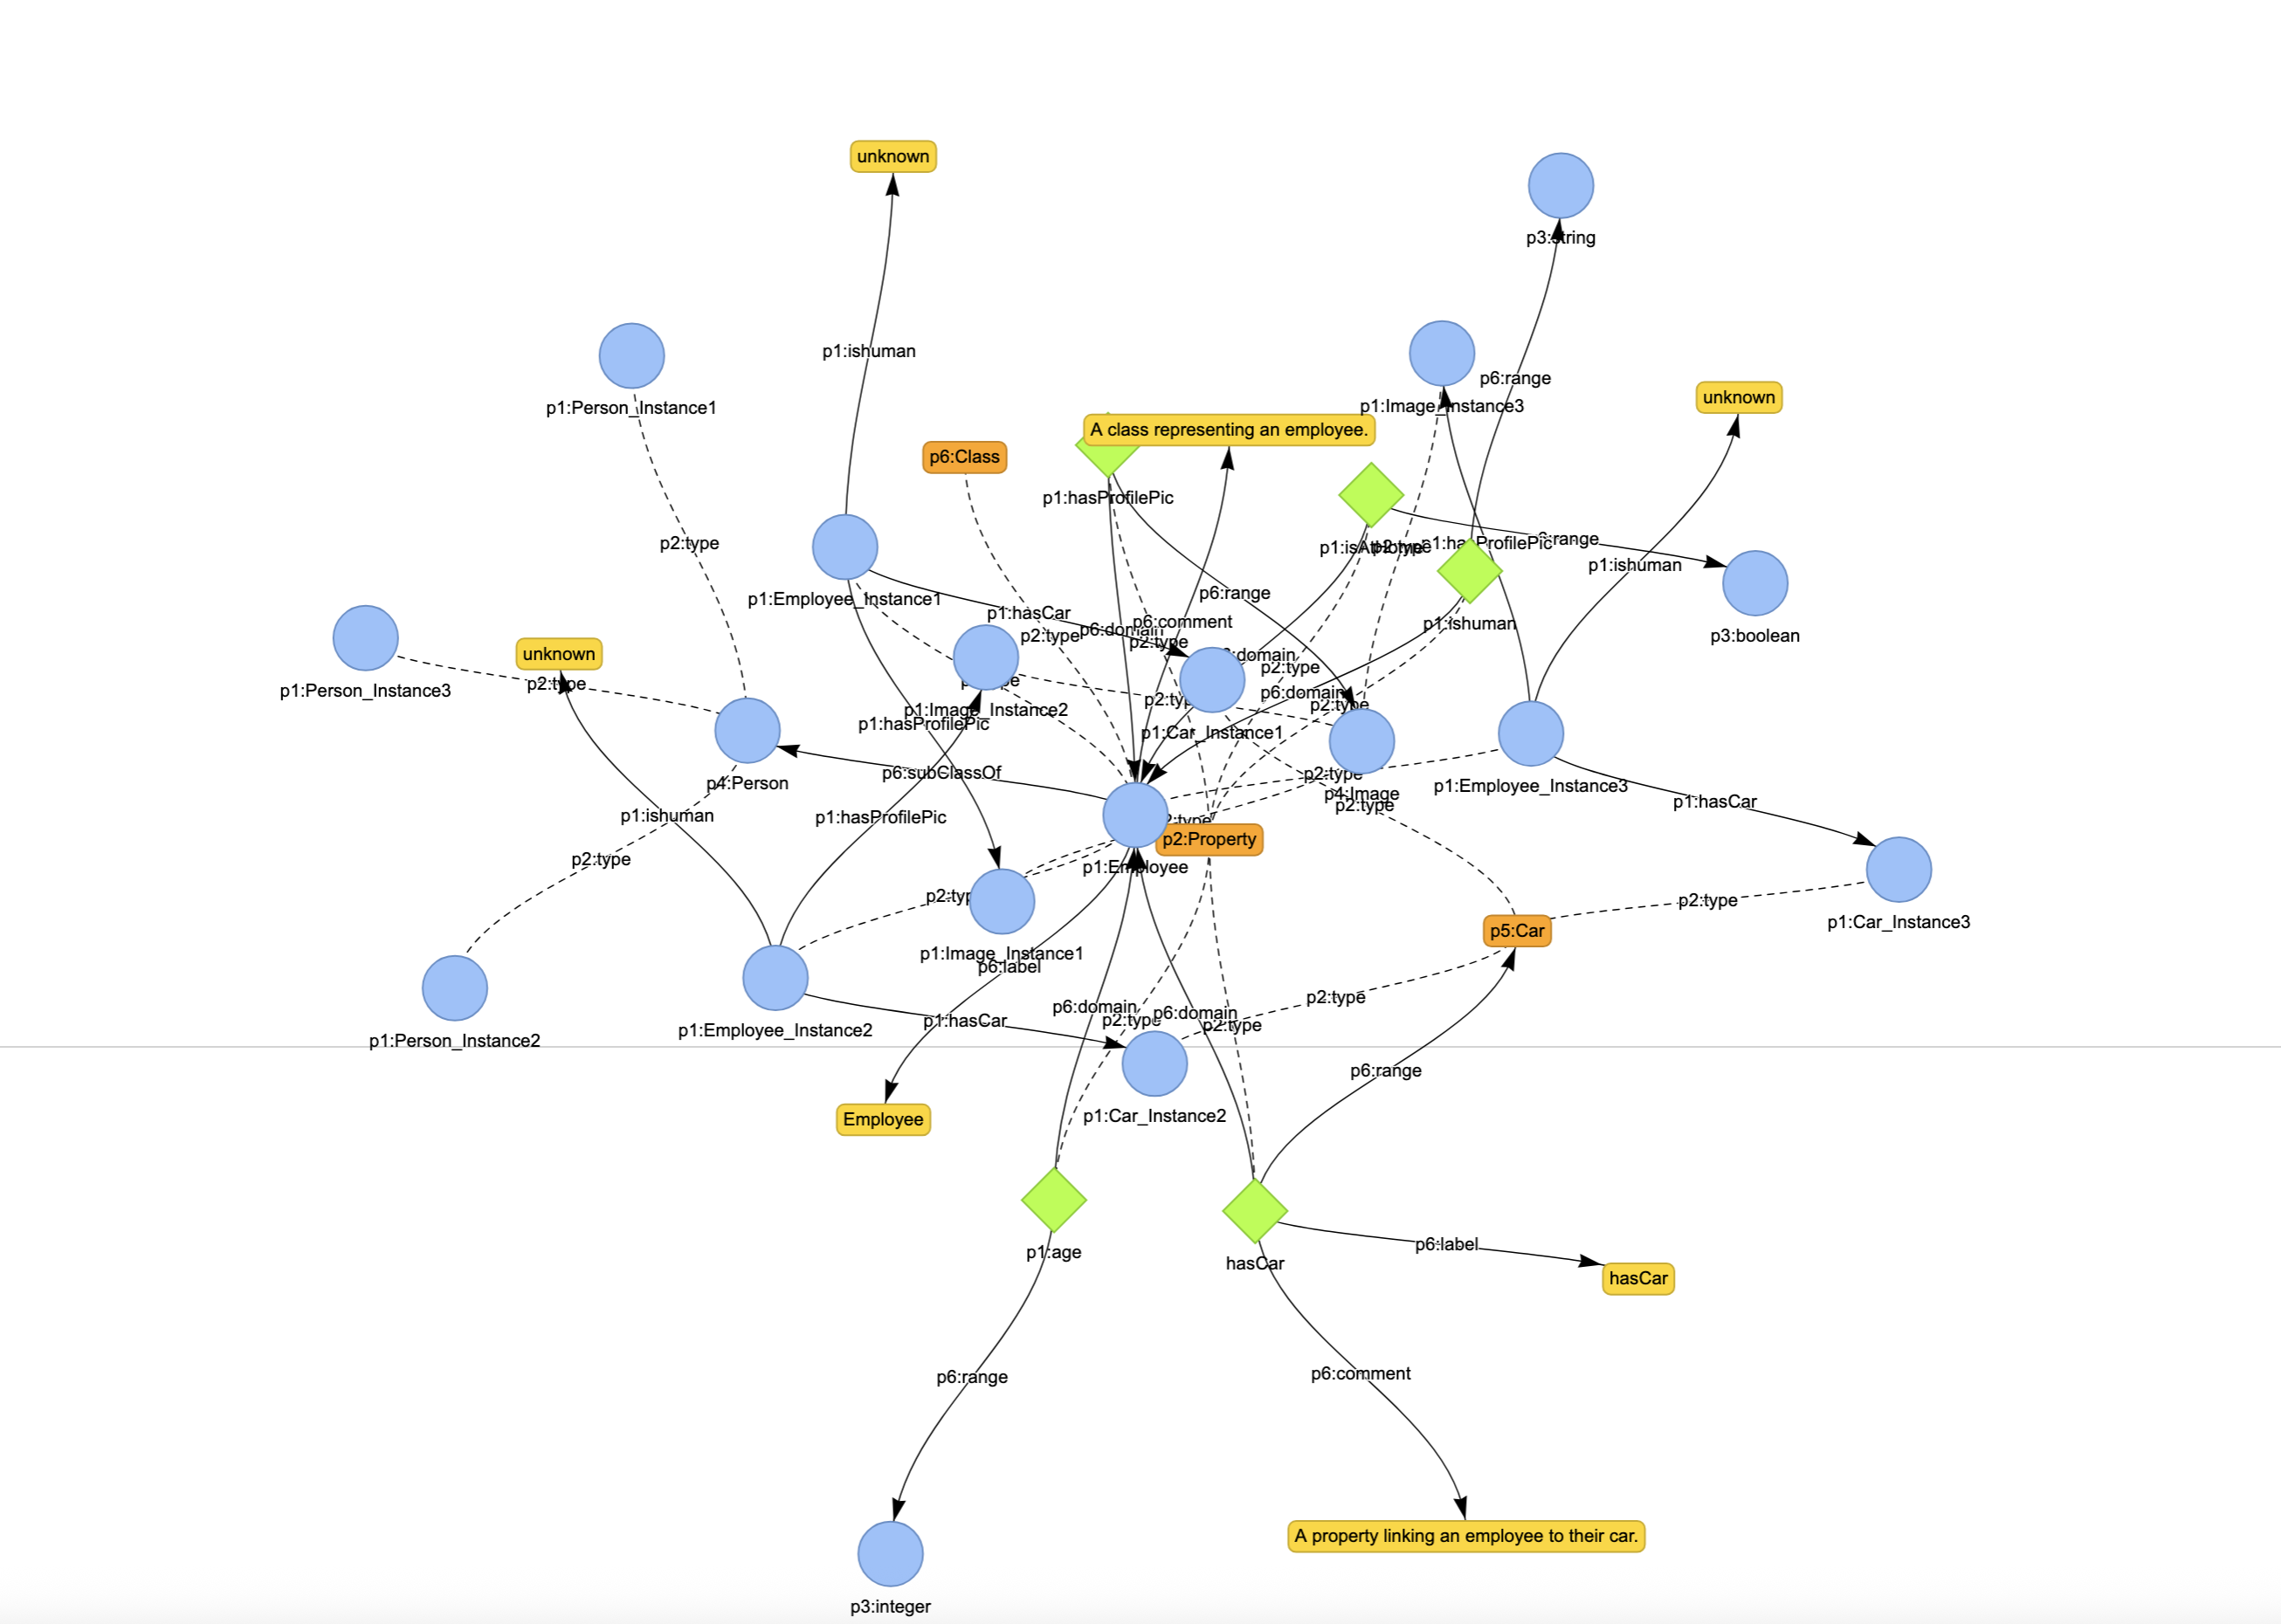
\includegraphics[width=14cm]{graphviewbrowserevaluation.png}
    \caption{Rending of the RDF graph}
    \label{fig:rendergraph}
\end{figure}

\paragraph{Comments}
For both the scenarios the graphs have been rendered correctly and no critical issues were found.
Unfortunately, I could find a way to stabilize the graph rendering in order to have the very same in the same place at each render. This would have help the user to better visualize the graph in case of some live edits in the RDF schema. 
\\
Some future work could include a better rendering engine and node distribution on the canvas.
% End 

% Start 
\subsection{RDF Graph and Schema Export}

\paragraph{Goal}
The next capability to evaluate is the \textbf{RDF Graph and Schema Export}. The user must be able to export the RDF schema and the generated graph.

\paragraph{Test Description}
To validate this functions, the following test scenarios were conducted:
\begin{itemize}
    \item \textbf{Test 3.1}: After the server response, a button allows to download the newly generated RDF schema - on Browser. 
    \item \textbf{Test 3.2}: After the server response, a button allows to visualize the newly generated schema in a new IDE window - on VSCode. 
    \item \textbf{Test 3.3}: After the server response, a button allows to export the RDF graph in a png format - on Browser. 
    \item \textbf{Test 3.4}: After the server response, a button allows to export the RDF graph in a png format - on VSCode. 
\end{itemize}

\subsubsection{Expected Result}

For two initial tests (\textbf{Test 3.1} and \textbf{Test 3.2}) scenario, the expected results are:
\begin{itemize}
    \item The correct generation of the download button.
    \item No anomalies in the download file. 
\end{itemize}

The remaining two tests (\textbf{Test 3.3} and \textbf{Test 3.4}), are expected to:
\begin{itemize}
    \item Generate a button that allow the graph to be exported in a PNG format. 
    \item The image graph in the PNG file is consistent with the one visualized in the application canvas.
\end{itemize}

\subsubsection{Actual Results}

The figure \ref{fig:schemadownload} showcase the first two test cases. The performed action has been marked with a red circle.
The outcome of the action is marked in a light green square. 

The figure \ref{fig:graphdownloadfrombrowsersandIDE} is the result of the last two test cases. The same marking process has also been in use in this figure.

All of them has been marked as passed.
\\

\begin{figure}[htb]
    \centering
    \begin{subfigure}[b]{0.48\textwidth}
        \centering
        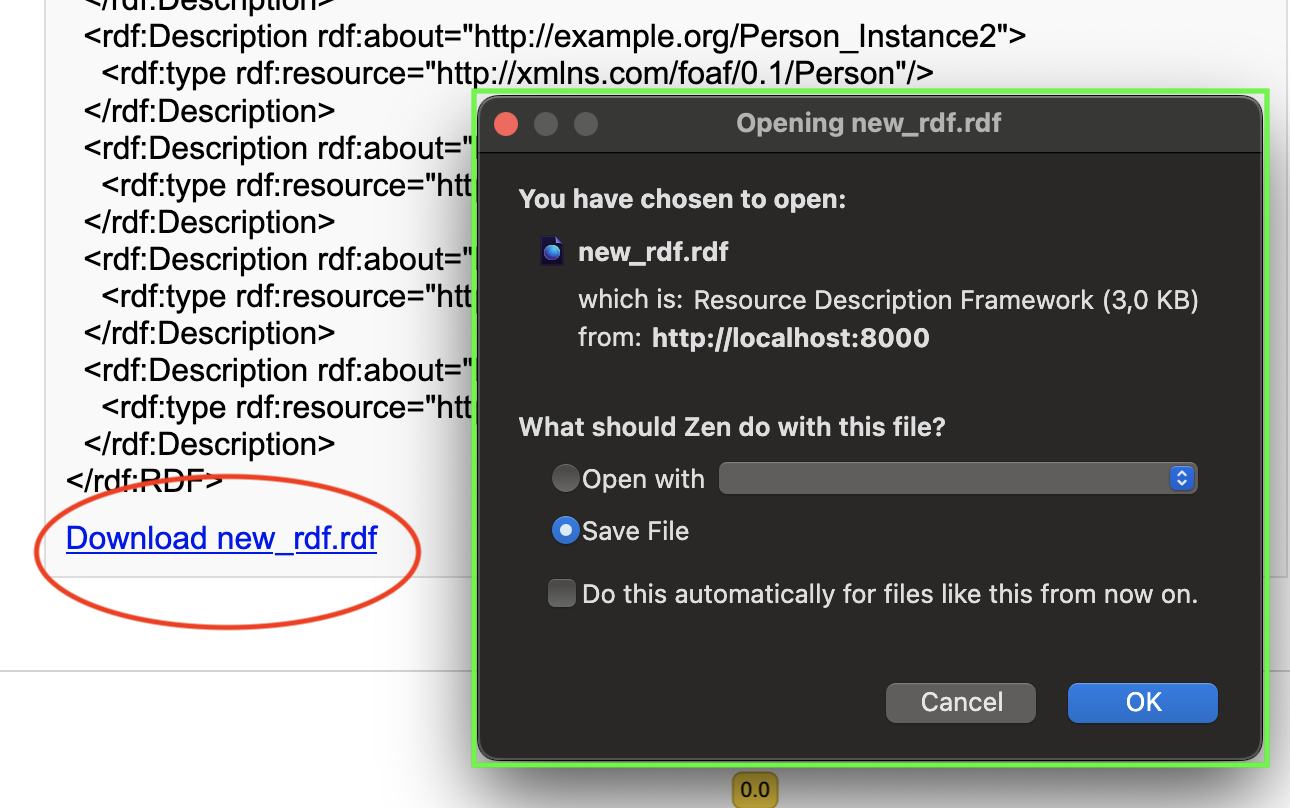
\includegraphics[width=\textwidth]{schemadownloadBrowser.png}
        \caption{Click action on the download button to download the RDF schema}
        \label{fig:RDFschemadownloadA}
    \end{subfigure}
    \hfill
    \begin{subfigure}[b]{0.48\textwidth}
        \centering
        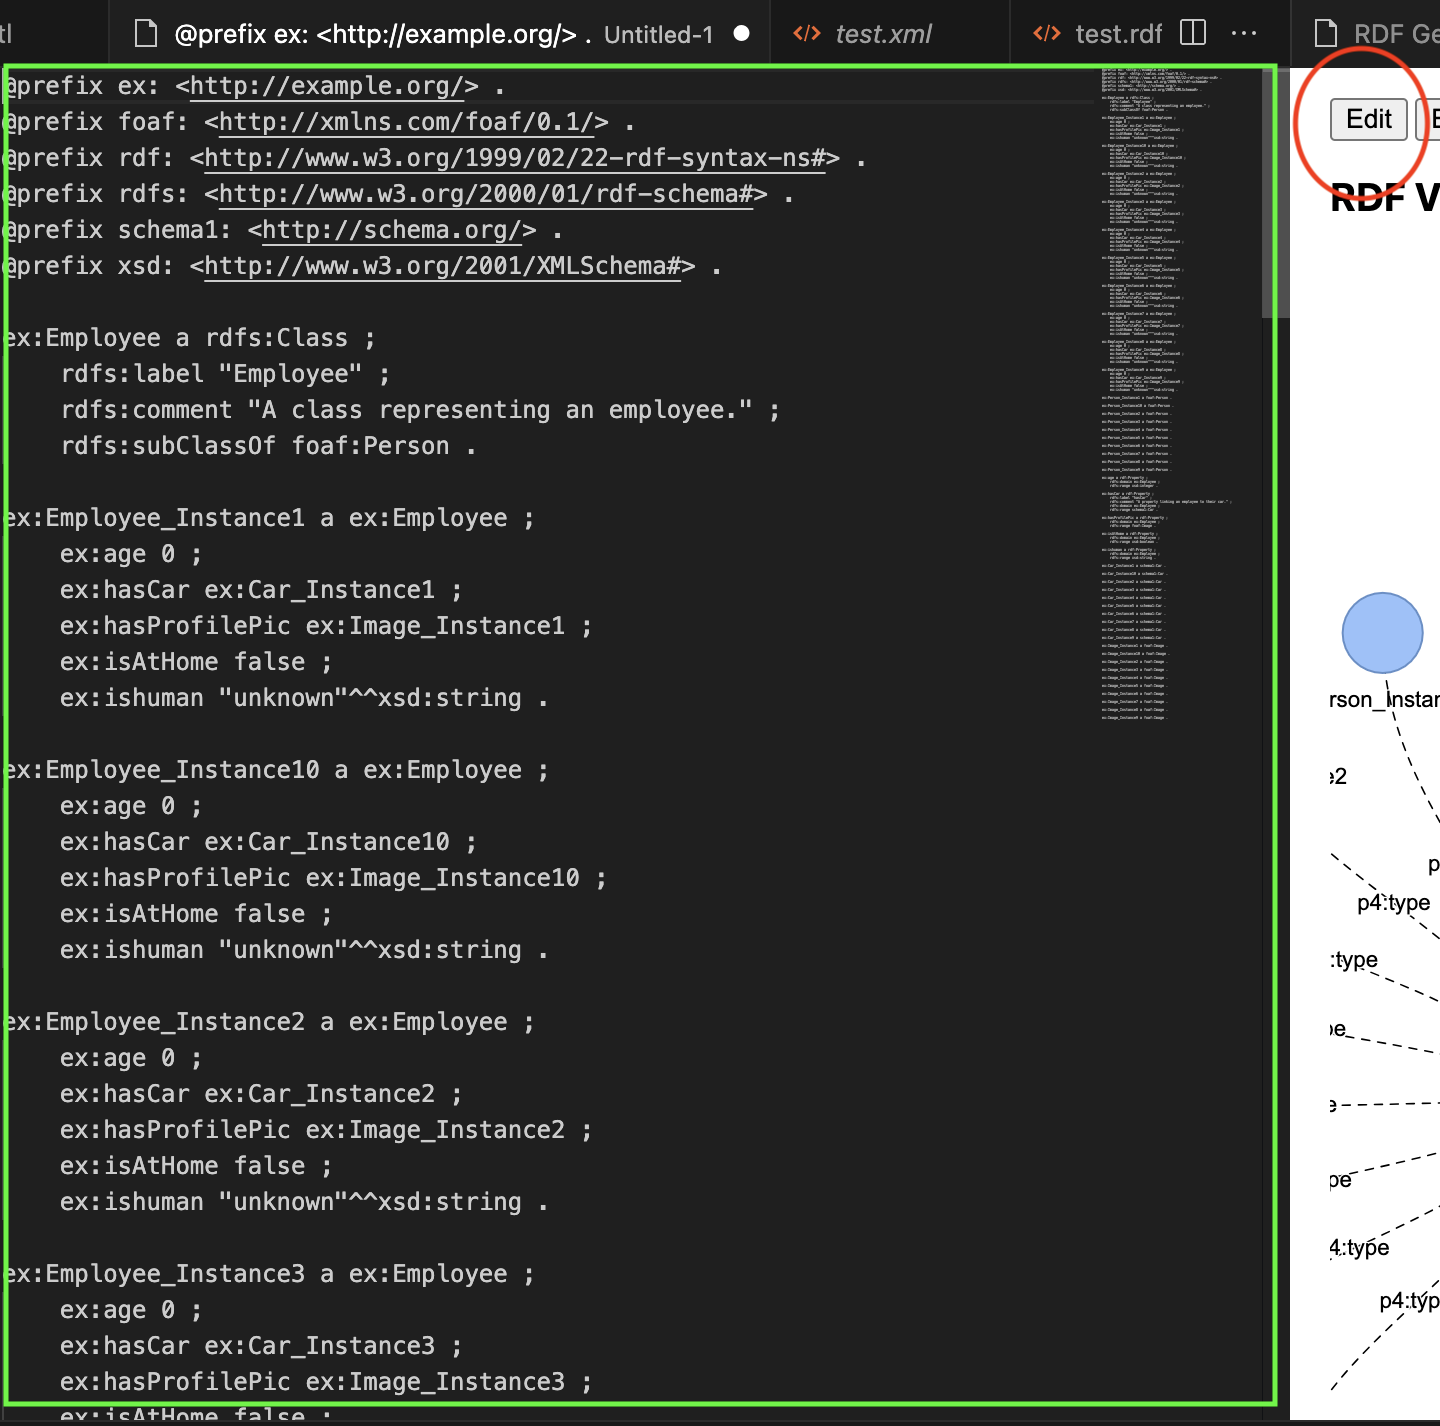
\includegraphics[width=\textwidth]{schemadownloadIDE.png}
        \caption{Click action on the edit button to download/edit the RDF schema}
        \label{fig:RDFschemadownloadB}
    \end{subfigure}
    \caption{RDF Schema download methods for Browsers client and IDE client}
    \label{fig:schemadownload}
\end{figure}

\begin{figure}[H]
    \centering
    \begin{subfigure}[b]{0.48\textwidth}
        \centering
        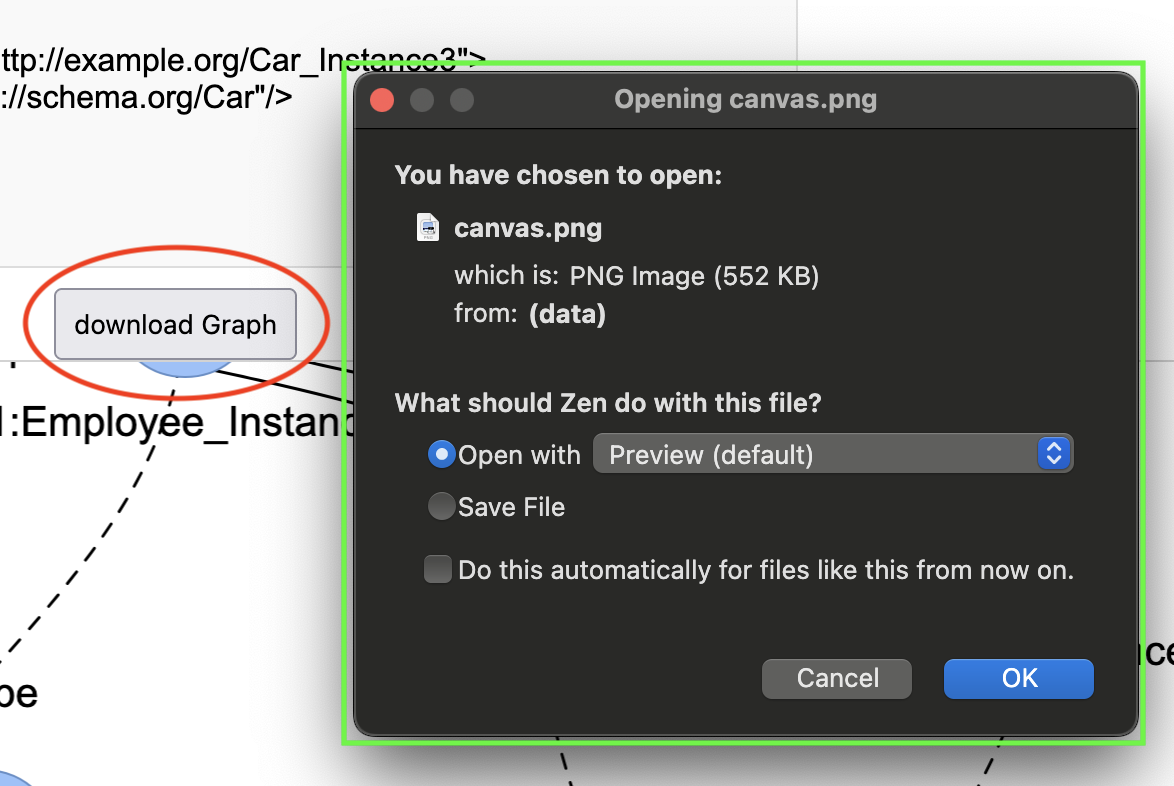
\includegraphics[width=\textwidth]{graphdownloadBrowser.png}
        \caption{Click action on the download button to download the RDF Graph}
        \label{fig:graphdownloadA}
    \end{subfigure}
    \hfill
    \begin{subfigure}[b]{0.48\textwidth}
        \centering
        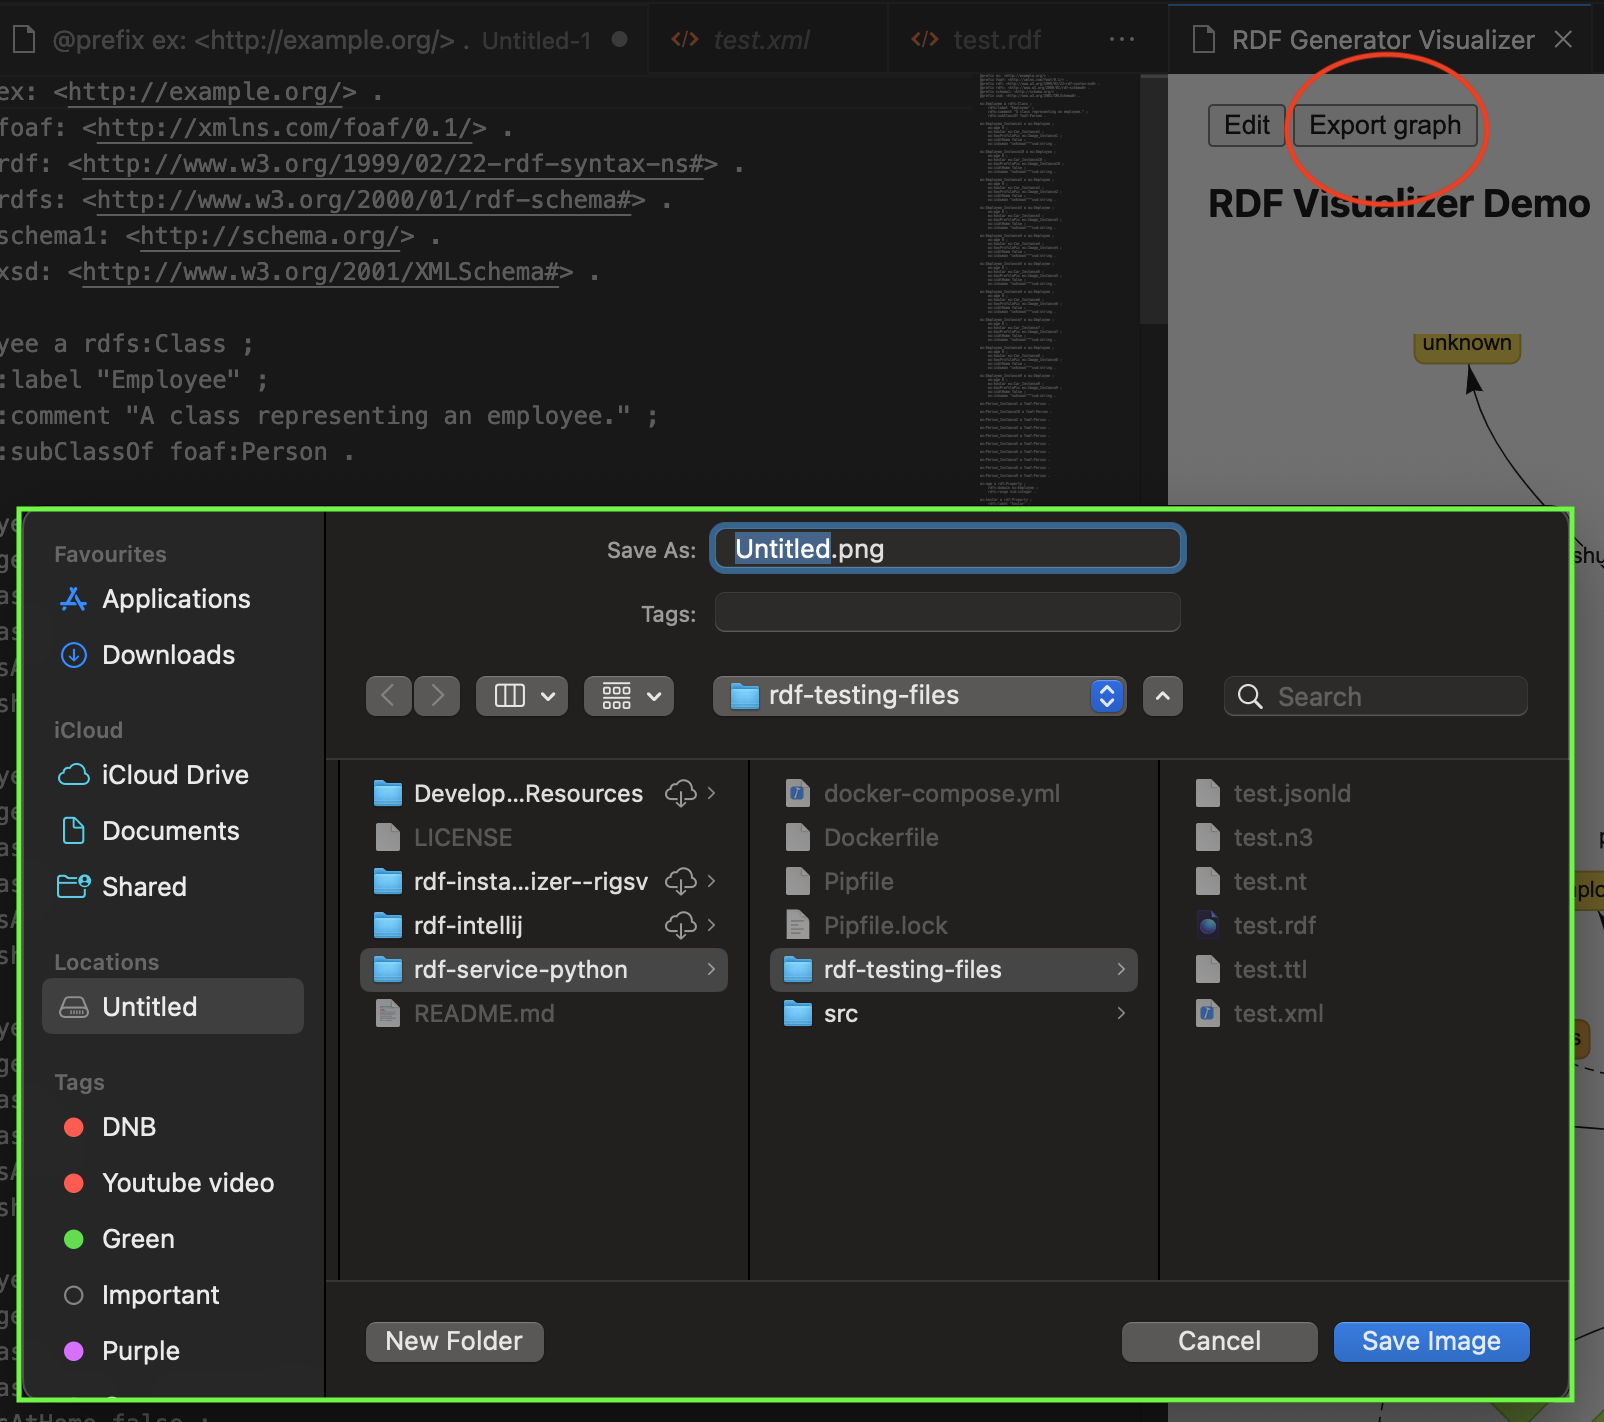
\includegraphics[width=\textwidth]{graphdownloadIDE.png}
        \caption{Rendering of RDF graph B}
        \label{fig:graphdownloadB}
    \end{subfigure}
    \caption{RClick action on the download button to download the RDF Graph}
    \label{fig:graphdownloadfrombrowsersandIDE}
\end{figure}


\paragraph{Comments}
All the test have passed and not critical issue were found the testing process.
Although one minore but has been found while testig the edit button in the IDE enviroment. 
\\
When the button is clicked and the schema is visualized in a new VSCode tab, if the user edits the file, it cannot be sent to the server directly. 
The file must be first saved and then sent to the server. Any action performed on a not saved file will cause the server to answer with an error. 

Future updated will provide a solution to the described bug and improvements in the RDF scheme edit mode, like allowing edits in the browser mode before the download and the options to re-render the graph automatically after a change in the file. 
% End 

\section{Performance Evaluation}
% Start Performance 1 
\subsection{Rendering Time}

\paragraph{Goal}
This test evaluates the responsiveness of the RDF visualization system by measuring the time required to render RDF graphs of increasing complexity. The rendering time is defined as the duration from server response to the completion of layout and DOM paint on canvas.

\paragraph{Method}
To test the rendering performance, three different schema sizes were generated:
\begin{itemize}
    \item \textbf{Small schema}: 10 instances generated
    \item \textbf{Medium schema}: 50 instances generated
    \item \textbf{Large schema}: 100 instances generated
\end{itemize}

Each rendering test was executed 3 times, and the average rendering time was recorded using \texttt{performance.now()} browser function.

\subsubsection{Results}

\begin{table}[H]
\centering
\begin{tabular}{|c|c|c|}
\hline
\textbf{Schema Size} & \textbf{Instances} & \textbf{Avg. Render Time (ms)} \\ \hline
Small & 10 & 121 \\ \hline
Medium & 50 & 4638 \\ \hline
Large & 100 & 9871 \\ \hline
\end{tabular}
\caption{Rendering time of RDF graphs with increasing complexity}
\label{tab:rendering-times}
\end{table}

\paragraph{Comments}
The results demonstrate a steep increase in rendering time with the number of nodes. While the small schema rendered almost instantly (121 ms), the medium and large schemas took 4.6 and 9.8 seconds respectively. This nonlinear growth in rendering time is attributed to the physics-based layout engine used by vis.js.

The delays observed in medium and large graphs can negatively affect user experience. To guarantee a nice UX the instances that can be generated are limited to a maximum number of ten. Future optimizations could include:
\begin{itemize}
    \item Reducing the number of stabilization iterations for larger graphs.
    \item Using simplified layouts (e.g., hierarchical layout).
    \item Introducing progressive or chunked rendering for large datasets.
\end{itemize}


\subsection{Instance generation time}

\paragraph{Goal}
This test evaluates the responsiveness of the RDF instance generation system (with no properties search) from the incoming request to the server response.

\paragraph{Method}
To test the rendering performance, three different schema sizes were generated:
\begin{itemize}
    \item \textbf{Small schema}: 10 instances generated
    \item \textbf{Medium schema}: 50 instances generated
    \item \textbf{Large schema}: 100 instances generated
\end{itemize}

Each generation test was executed 3 times, and the average response time was recorded using the \texttt{Time} python library.

\subsubsection{Results}

\begin{table}[H]
\centering
\begin{tabular}{|c|c|c|}
\hline
\textbf{Schema Size} & \textbf{Instances} & \textbf{Avg. Render Time (ms)} \\ \hline
Small & 10 & 36.2 \\ \hline
Medium & 50 & 98.0 \\ \hline
Large & 100 & 142.22 \\ \hline
\end{tabular}
\caption{Response time of RDF instance generator function with increasing complexity}
\label{tab:rendering-times}
\end{table}

\paragraph{Comments}
The results indicate that the instance generation time increases moderately with the number of instances requested. The small schema completed generation in approximately 36 ms, while the medium and large schemas required 98 ms and 142 ms respectively. Although the growth is not exponential, the system's responsiveness could degrade if the quality of the hardware is lowered.

To ensure a consistently smooth user experience, be coherent with the current graph visualization limit and avoid potential performance bottlenecks for machine with a low budget hardware, the current implementation limits instance generation to a maximum of ten instances per request. 

Future enhancements may explore asynchronous processing, or batched generation to support larger requests without compromising server responsiveness.
\\
\\
\subsection{Instance generation time with property search}

\paragraph{Goal}
This test evaluates the responsiveness of the RDF instance generation system, with properties search, from the incoming request to the server response.

\paragraph{Method}
To test the rendering performance, three different schema sizes were generated:
\begin{itemize}
    \item \textbf{Small schema}: 1 instances generated
    \item \textbf{Medium schema}: 5 instances generated
    \item \textbf{Large schema}: 10 instances generated
\end{itemize}

Each generation test was executed one time only to not stress the LOV api service with testing request, and the average response time was recorded using the \texttt{Time} python library.

\subsubsection{Results}

\begin{table}[H]
\centering
\begin{tabular}{|c|c|c|}
\hline
\textbf{Schema Size} & \textbf{Instances} & \textbf{Avg. Render Time (ms)} \\ \hline
Small & 1 & 206592 \\ \hline
Medium & 5 & 215507\\ \hline
Large & 10 & 245350 \\ \hline
\end{tabular}
\caption{Response time of RDF instance generator function with propertiesn search}
\label{tab:rendering-times}
\end{table}

\paragraph{Comments}
The results reveal a surprising insight: the number of instances requested had minimal influence on the overall generation time. Instead, the dominant factor affecting performance was the number of properties that required semantic enrichment with the vocabulary lookup, specifically those whose ranges point to other classes.

This is explained by the fact that, for each such property, the system performs a query against the Linked Open Vocabularies (LOV) API to search for semantically relevant property names. As the number of properties requiring lookup increases, so does the total response time, regardless of the number of instances being generated.

Due to this dependency on an external service and its associated latency, the current implementation limits instance generation with property search to a maximum of 3 instances with only 1 property enhancements per class. This helps reduce the number of API calls and ensures acceptable response times. 

Future improvements may include result caching, local vocabulary indexing and batching to enhance performance. 

% edge cases analysis
\subsection{Edge Case Analysis}

\paragraph{Goal}
This section evaluates how the system handles unexpected input scenarios that may occur during RDF instance generation. The objective is to ensure robustness and graceful failure handling, even when inputs deviate from normal expectations.

\paragraph{Method}
A series of edge case tests were conducted to assess the stability and correctness of the system in the following situations:

\begin{itemize}
    \item \textbf{Invalid file:} The input file is not an rdf file
    \item \textbf{Empty Schema:} Schema with no classes or properties defined.
    \item \textbf{Circular Class References:} A Class (A) has a property pointing to another Class (B), which points back to the previous Class.
    \item \textbf{Unsupported RDF Constructs:} Use of blank nodes or advanced RDF syntax that has not specifically handled.
    \item \textbf{Highly Connected Schema:} A class with more than 20 properties linking to multiple other classes.
    \item \textbf{Malformed Input:} Invalid RDF syntax.
\end{itemize}

Each scenario was executed through the instance generator and monitored for application stability, error messages, and correctness of the output.

\paragraph{Results}
The application performed robustly in most edge case scenarios. Table~\ref{tab:edge-case-results} summarizes the outcomes.

\begin{table}[H]
\centering
\begin{tabular}{|p{4.5cm}|p{3cm}|p{6cm}|}
\hline

\textbf{Test Case} & \textbf{Status} & \textbf{Notes} \\ \hline 
Invalid file & Partial & Server returned a generic error response (\textit{Error loading content}). \\ \hline
Empty Schema & Pass & Server returned an empty canvas with no errors. \\ \hline
Circular Class References & Pass & Instance generation completed; circular references were handled without infinite loops. \\ \hline
Unsupported RDF Constructs & Pass & Blank nodes were handled without failure; no warning issued. \\ \hline
Highly Connected Schema & Partial & Significant performance degradation observed in the rendering of the graph. \\ \hline
Malformed Input & Partial & Server returned a generic error response (\textit{Error loading content}). \\ \hline
\end{tabular}
\caption{Summary of edge case testing outcomes}
\label{tab:edge-case-results}
\end{table}

\paragraph{Comments}
The system demonstrates strong resilience against most edge cases. In particular, circular class references and highly nested schemas did not lead to crashes or infinite loops. However, two weak points were identified: the invalid file and malformed input.
Addressing these cases would improve user experience and system robustness.